% import.tex - Examples of importing .eps files into a Latex document

% Andrew Roberts - September 2003
% Last updated: 5th November 2011
% Last update by John Minter 2021-05-30 to use chick-img.png

\documentclass[english]{article}

\usepackage{times}
\usepackage{babel}
\usepackage{graphicx}

\begin{document}

\title{Getting to Grips with \LaTeX{} --- Importing Graphics}
\author{Andrew Roberts}
\maketitle

An example of an imported image:

\begin{center}
  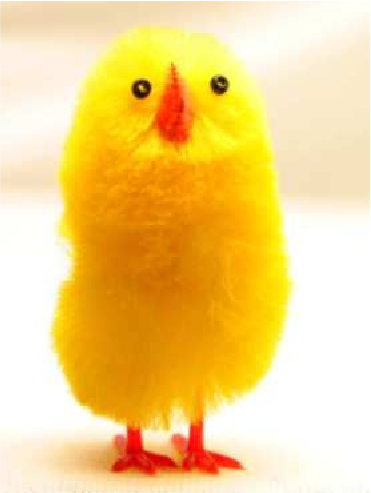
\includegraphics{chick-img.png}
\end{center}

However, it is too large, so scale it down within \LaTeX{} using the
\texttt{scale} parameter, which scales by a constant
scale factor (0.5, for example, to reduce by half):

\begin{center}
  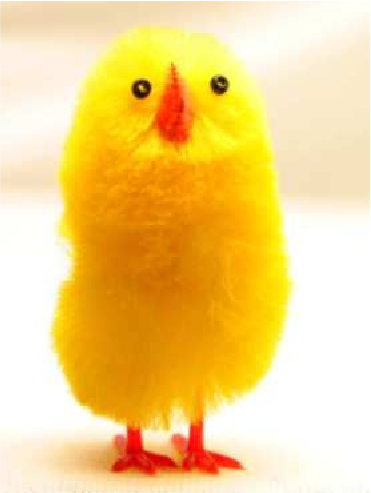
\includegraphics[scale=0.5]{chick-img.png}
\end{center}

Alternatively, you can specify lengths for the image to be resized.  The
\texttt{width} and \texttt{height} parameters are the ones you need.  If
you only specify one of the parameters, the aspect ratio will be
maintained.  For example, \texttt{width=2.5cm}:
\begin{center}
  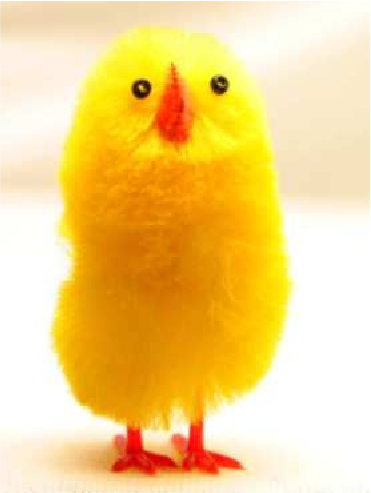
\includegraphics[width=2.5cm]{chick-img.png}
\end{center}

Other tricks up graphicx's sleeves include the ability to rotate
(\texttt{angle=180}).

\begin{center}
  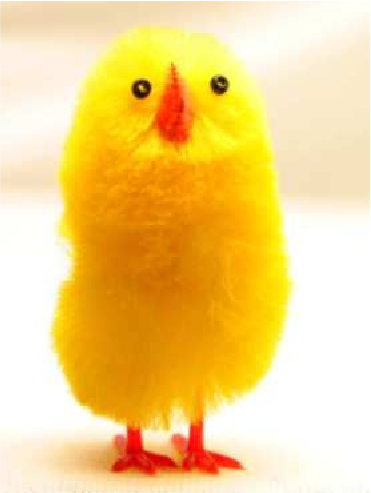
\includegraphics[scale=0.5, angle=180]{chick-img.png}
\end{center}

And it is possible to focus in on a particular region of interest.
Admittedly, it can often require a little trial-and-error. Using
\texttt{trim = left bottom right top} crops the amount specified from
the edge of the image.  Remember to set the \texttt{clip} parameter too.

\begin{center}
  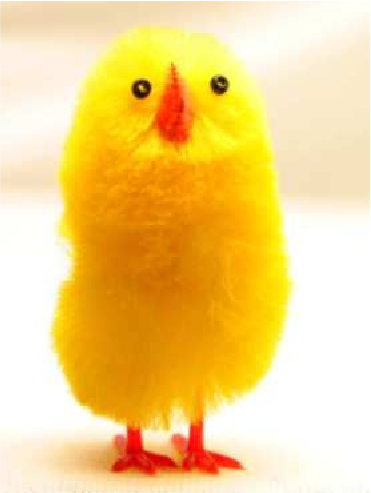
\includegraphics[trim = 10mm 80mm 20mm 5mm, clip, width=3cm]{chick-img.png}
\end{center}




\end{document}